\subsection{Comparative Analysis} \label{comparative_analysis}
In this subsection we consider a comparative analysis of mentioned methodologies to discern the most suitable approach for our specific context.

In the context of evaluating three approaches (Visual Narrator, GPT-3.5, and Conditional Random Fields or CRF) for the task of domain concept extraction from a corpus of stories, it is evident that CRF emerges as a compelling choice. Here are the reasons why CRF should be chosen for our approach:
\begin{itemize}
\item Tailored Approach: Mosser et al. highlights CRF as a rule-based approach, allows for a tailored and domain-specific model. This tailored approach is crucial when dealing with complex domain-specific tasks like concept extraction. CRF can be fine-tuned by domain experts to address the specific challenges of the task.
\item Training Requirement: CRF requires training, it was trained using a classical 80/20 separation method. This training phase allows CRF to learn the patterns and relationships between domain concepts and the textual context. This training can lead to improved accuracy and relevance in domain concept extraction (Figure \ref{fig:coparing_approaches}) \cite{arulmohan2023extracting}.
\item Model Complexity: In comparison to other approaches, CRF's implementation is relatively simple, and it requires a smaller codebase. This simplicity makes it easier to manage and maintain, reducing the complexity associated with more extensive models like GPT-3.5.
\item $F-measure\ (F_1)$ : Mosser et al. measures performance using the $F_1$ score, which is particularly suitable for this task. $F_1$ considers both precision and recall, which is essential when dealing with domain concept extraction. It is well-suited for situations where false positives and false negatives have different costs \cite{arulmohan2023extracting}.
\item Superior Performance: Empirical results indicate that CRF consistently outperformed other approaches, including GPT-3.5, in all evaluation criteria. CRF achieved the highest $F_1$ scores, particularly for Persona's extraction, reaching a perfect score of 1.0 which means a perfect match (score of 0.0 means that precision or recall is null). This superior performance is indicative of CRF's effectiveness in this specific task \cite{arulmohan2023extracting}.
\item Reproducibility: CRF offers transparency and interpretability, making it easier to understand and reproduce results compared to more opaque machine learning models.
\item Concerning the Agile DevOps Paradigms: Visual Narrator keeps its conceptual model internal and exposes black-box analysis to users, dedicated to stories quality in terms of requirements engineering, for example. Thus, it does not support the DevOps team in the development, as the provided feedback focuses on the requirements expression instead of their role in the software development. CRF instead leverage the graph structure of the ontologies and exploit a graph-based meta-modelling and compositional approach to shorten the feedback loop between developers and Ops while supporting agile development’s iterative and incremental nature \cite{mosser2022modelling}.
\item Syntactic and semantic Covering: In contrast to GPT-3.5 and CRF, which consider both the syntactic and semantic aspects of US, NLP has constrained its focus solely to the syntactic structure of the US.
\end{itemize}
\begin{figure}
\center
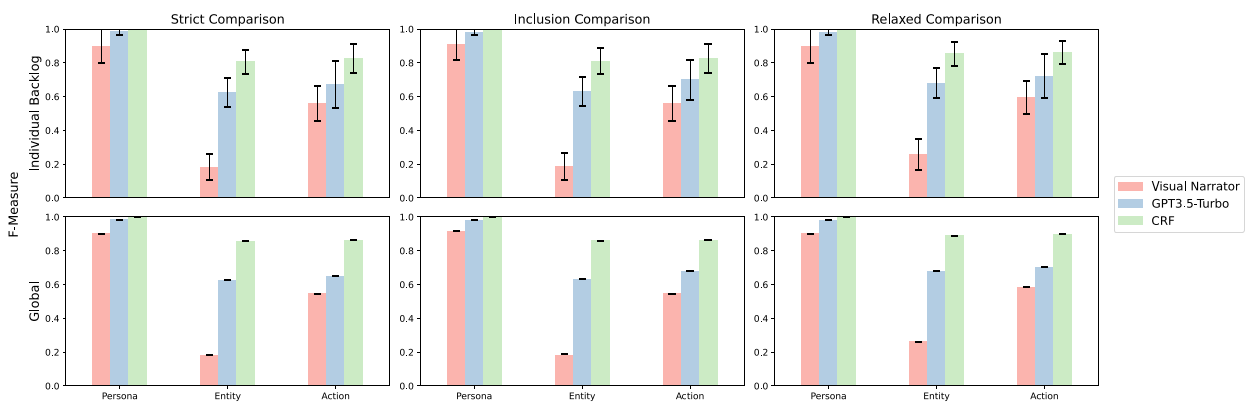
\includegraphics[width=\textwidth, height=5.76cm]{Comparing_approaches_to_the_ground_truth}
\caption{Comparing approaches to the ground truth: $F-measure \ (F_1)$ results for Visual Narrator, CRF and GPT-3.5  \cite{arulmohan2023extracting}}\label{fig:coparing_approaches}
\end{figure}
\subsection{Bottom Line}\label{crf_bottom_line}
We have chosen the Conditional Random Fields (CRF) approach because of their graph-based nature and their significant promise in terms of precision and recall, which is particularly important in the context of domain concept extraction. CRF can cover both syntactic and semantic aspects, especially when complemented by an appropriate conceptual metamodel, which makes it suitable for definition as a type graph in Henshin. The annotations generated by CRF can then be used for transformation into a rule-based graph transformation system, improving support for DevOps practices.


